%Description, implementation, alignment corrections, performance and latencyFigure\,\ref
%%%%%%%%% Sample inclusion of a figure
 % \begin{figure}[h]
 % \begin{center}
 % \includegraphics[width=0.8\textwidth]{algorithms-saclay/Plot1}
 % \caption{Caption of plot 1}
 % \label{fig:Monitoring}
 % \end{center}
 % \end{figure~\ref{fig:}}
%%%%%%%%%%%%%%%%%%%%%%
\FloatBarrier
 \subsubsubsection{Principle of the algorithm}
%%%%%%%%%%%%%%%%%%%%%%
The eight MM layers that form a large sector are numbered from 1 to 8 (1, 2, 5 and 6 being the $X$ layers, 3 and 7 the $U$ layers, and 4 and 8 the $V$ layers) and grouped in pairs: $(1, 5), (2, 6), (3, 7), (4, 8), (1, 6)$ and $(2, 5)$, so six pairs in total. When a muon passes through the detector, hits are created on each of the layers. For each considered pair, the first strips that triggered  for both layers of the pair are used to calculate the corresponding slope with the formula:
$${\rm slope_{pair}}=\frac{y_{\rm layer2}- y_{\rm layer1}}{z_{\rm layer2}- z_{\rm layer1}}$$
where $y_{\rm layer1,2}$ and $z_{\rm layer1,2}$ are the strip positions in the $(y,z)$ plane. Figure\,\ref{fig:SaclayTriggerPrinciple} illustrates the pair selection and the angle calculation with respect to the interaction point (IP). The distance between layer pairs (1,\,5), (2,\,6), (3,\,7) and (4,\,8) is of 126\,mm, 137\,mm for pair (1, 6) and 115\,mm for pair (2, 5) respectively as shown in Figure\,\ref{fig:SaclayAlgorithmPair}.

%%%%%%%%%%%%%%%%%%%%%%
 \begin{figure}[htb!]
  \begin{center}
  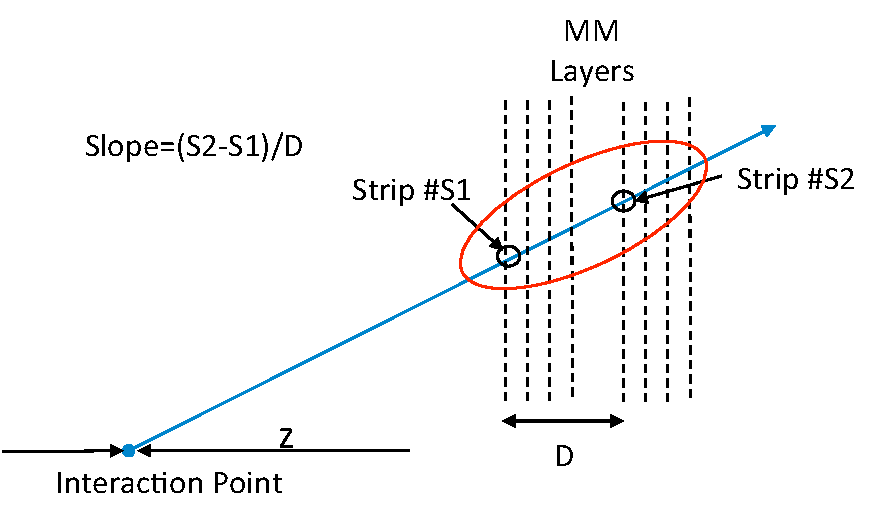
\includegraphics[width=0.5\textwidth]{algorithms-saclay/SaclayTriggerPrinciple.pdf}
  \caption{Illustration of pair selection and angle calculation with respect to the interaction point.}
  \label{fig:SaclayTriggerPrinciple}
  \end{center}
  \end{figure}
%%%%%%%%%%%%%%%%%%%%%%
 \begin{figure}[htb!]
  \begin{center}
  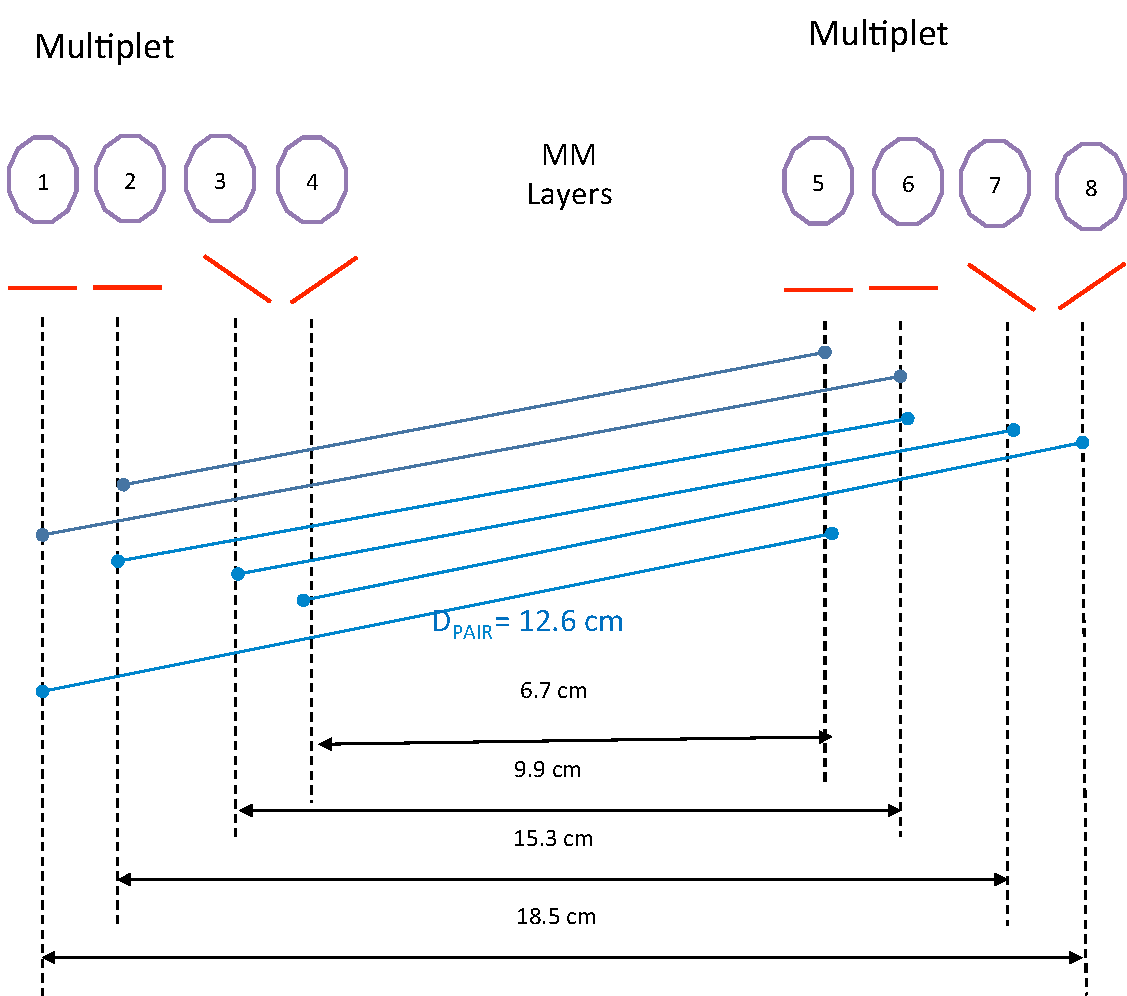
\includegraphics[width=0.55\textwidth]{algorithms-saclay/SaclayAlgorithmPair.pdf}
  
\includegraphics[width=0.7\textwidth]{algorithms-saclay/SaclaySlopeComaprison.pdf}
  \caption{Representation of pairs formed by the algorithm (top) and comparison between the slopes (bottom).}
  \label{fig:SaclayAlgorithmPair}
  \end{center}
  \end{figure}
%%%%%%%%%%%%%%%%%%%%%%
The so calculated slopes are then compared to each other as  shown in Figure\,\ref{fig:SaclayAlgorithmPair}. If a certain number of them (above some threshold value defined in the selection logic) are equal within a given precision, they are considered as forming a unique track corresponding to one muon and retained for further processes. All these calculations are done locally; the condition of a pointing track (i.e.\ coming from the interaction point) is then added in order to determine the Regions of Interest (RoI).

In this study, the detector is segmented in several panel regions which correspond originally to the segmentation in four chambers. With the present design, with only two chambers, the panels correspond to the logical segmentations (for instance, two or more panel or regions per chamber).
Figure\,\ref{fig:SaclayElectronicImplementation} shows the electronic implementation of the trigger for two bunch crossings (BC) for one panel region.
In order to allow for noise, multiple hits and multiple muons in a given panel region, up to 8 hits per layer and per BC can be considered by the algorithm. Hence, for each layer pair, a maximum of $8\times 8=64$ slopes is calculated. For 2~BC there are 4 sets of 6 layer pairs with 64 slopes calculation for each pair.
The algorithm described above intervenes at the ``SLOPE SELECT'' step in Figure\,\ref{fig:SaclayElectronicImplementation}, pre-selecting the track candidate for further processing. Performance and latency are also given in Figure\,\ref{fig:SaclayElectronicImplementation} assuming 320\,MHz tic frequency.
%%%%%%%%%%%%%%%%%%%%%%%
 \begin{figure}[htb!]
  \begin{center}
  
\includegraphics[width=0.98\textwidth]{algorithms-saclay/SaclayElectronicImplementation.pdf}
  \caption{Electronic implementation for one panel region.}
  \label{fig:SaclayElectronicImplementation}
  \end{center}
  \end{figure}
%%%%%%%%%%%%%%%%%%%%%%
%%%%%%%%%%%%%%%%%%%%%%
 \subsubsubsection{Algorithm Implementation}
%%%%%%%%%%%%%%%%%%%%%%
The algorithm performance is essential to respect the requirements on the trigger response time: a decision has to be made in less than 100\,nanoseconds. So to limit the number of calculations, the solution of a Look Up Table (LUT) has been retained. Its operating principle is as follows. \\
For each layer pair, a panel region  corresponds to a given range aperture angles from the IP as illustrated in Figure\,\ref{fig:SaclayAngleAperture}. These  aperture angles are delimited by the borders between the adjacent panel regions.
Based on simple geometrical considerations, it is possible to store all the possible values of the slopes (difference between strip numbers of the two layers) that a pointing track can have in a given panel region with a certain granularity in a 32 bits register.
Then for each layer pair, a Look Up Table is used to check  whether each of the 64 slopes is within the range of allowed values for this panel as presented in Figure\,\ref{fig:SaclayLUTprinciple}. As an output, each time a matching is found,  a bit  is filled in a 32-bit register which corresponds to the slope value.  Bit 0 is filled in case of no-match. For each layer pair, there are four such registers  corresponding to the four possible BC combinations. \\
In the following step of ``Slope Select Logic'' in Figure\,\ref{fig:SaclayElectronicImplementation}, the registers corresponding to the six layer pairs are compared. If there are minimum number of compatible values within a given precision (for example within two slope bits),  the combination is considered as valid and is kept for further process.  The track candidate slope is then determined by the average slope of the accepted segments. Track constraint to the IP could be implemented in the future.

In order to account for the larger distance from the IP of the second multilayer, projective panel region are defined which are slightly different from the physical  segmentation. The principle is depicted on Figure\,\ref{fig:SaclayProjectivePR}.
%%%%%%%%%%%%%%%%%%%%%%%
 \begin{figure}[htb!]
  \begin{center}
  
\includegraphics[width=0.65\textwidth]{algorithms-saclay/SaclayAngleAperture.pdf}
  \caption{Angle aperture for different panel regions.}
  \label{fig:SaclayAngleAperture}
  \end{center}
  \end{figure}
%%%%%%%%%%%%%%%%%%%%%%%%
%%%%%%%%%%%%%%%%%%%%%%%
 \begin{figure}[htb!]
  \begin{center}
  
\includegraphics[width=0.65\textwidth]{algorithms-saclay/SaclayLUTprinciple.pdf}
  \caption{Operating principle of the LUT.}
  \label{fig:SaclayLUTprinciple}
  \end{center}
  \end{figure}
%%%%%%%%%%%%%%%%%%%%%%%%
%%%%%%%%%%%%%%%%%%%%%%%
 \begin{figure}[htb!]
  \begin{center}
  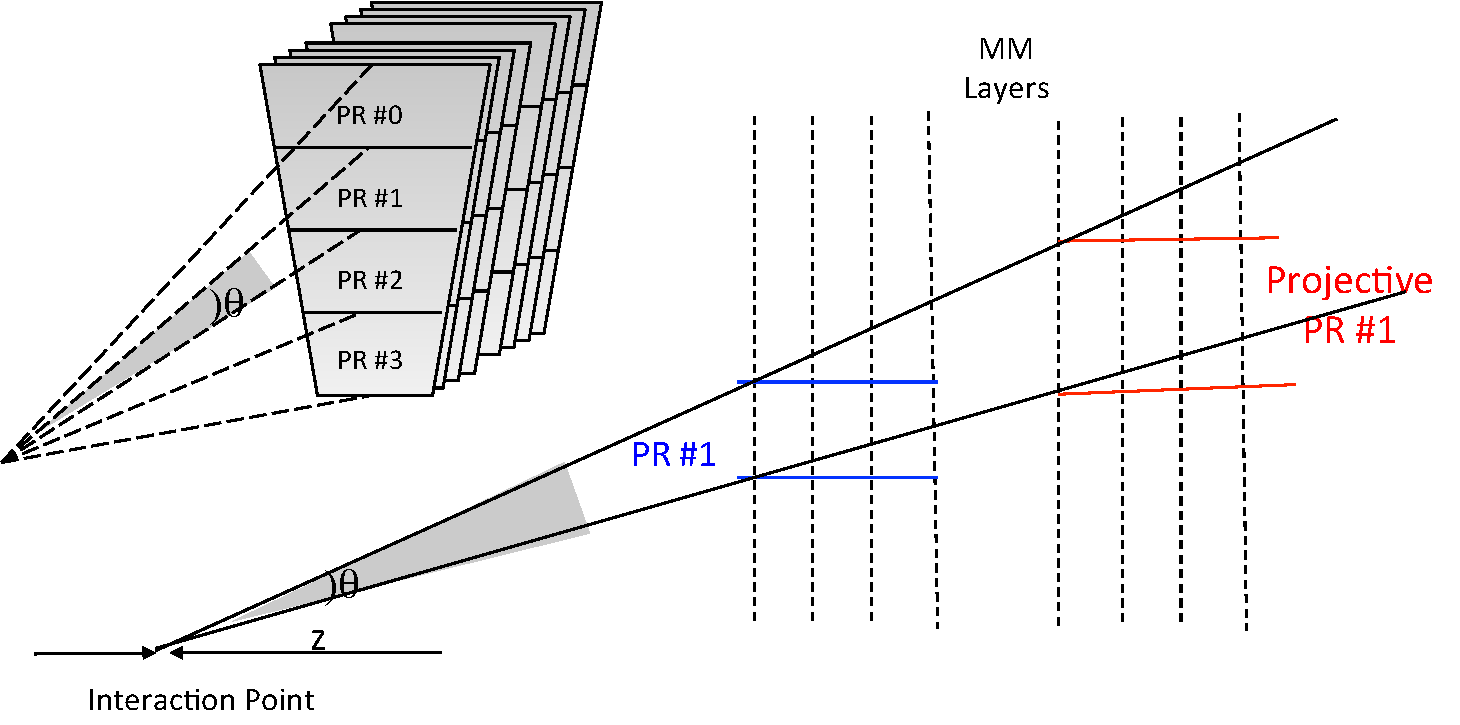
\includegraphics[width=0.7\textwidth]{algorithms-saclay/SaclayProjectivePR.pdf}
  \caption{Implementation of projective panel regions.}
  \label{fig:SaclayProjectivePR}
  \end{center}
  \end{figure}
%%%%%%%%%%%%%%%%%%%%%%%%
%\textbf{Construction of the Look Up Table} : The first step to construct the LUT is to determine the angles delineating the four panel regions. To do so, the simulation has been used to identify the $y$-coordinates where hits are missing, i.e. the boundaries between the panel regions. Their analysis allows to determine their corresponding angles from the IP by the formula $\theta_{d}=\frac{y_{\rm layer0}}{z_{\rm layer0}}$ and the corresponding slopes of these angle given by their tangents $\tan(\theta_{d})$. The aperture angle $\theta_{d}$ should be slightly different for each layer because of the different distances from the IP; but it has been observed that these differences are too small (the layers are distant of a few centimeters from each other and about seven meters from the IP) to change the results so they are considered as negligible.
%
%The Table~\ref{tab:NsLUT}The aperture angles obtained thanks to these informations for each panel regions and the numbers of strips $N_{s}$ corresponding to these aperture angles are grouped in the Table~\ref{tab:NsLUT}. The formula used is:
%$$N_{s}=\frac{D_{2} }{ l_{p}}=D_{pair}\times \frac{\tan(\theta_{dfi}) - \tan(\theta_{dsi})}{l_{p} }$$
%where $i$ vary from 0 to 3 for the angles of the dead zones, and where $D_{2}$ is depicted in Figure\,\ref{fig:SaclayAngleAperture}. $l_{p}$ is
%the pitch between the beginning of strip and the beginning of the following one, and $D_{pair}$ is the distance between the two layers of the pair.

\textbf{Construction of the Look Up Table} : the aperture angles are obtained from the simulation as shown in Figure\,\ref{fig:SaclayAngleAperture}. The Table~\ref{tab:NsLUT} gives these aperture angles as well as the expected maximum value of difference of slopes expressed in term of number of strips  ($N_{s}$ ).
$N_{s}$ depends of the distance between the two layers of the pair; the numbers given in the Table\,\ref{tab:NsLUT} are for the pairs of 126~mm distance. These numbers are slightly smaller for the pair of 115\,mm and slightly higher for the pair of 137\,mm.

%%%%%%%%%%%%%%%%%
\begin{table}[h!tbp]
\centering
\begin{tabular}{ c  c  c }
\toprule
Panel region & Aperture angle ($^{\circ}$) & Number of strips ($N_{s}$) \\
\midrule
0 & 4.73 & 31\\
1 & 5.93 & 36\\
2 & 6.45 & 36\\
3 & 6.86 & 36\\
\bottomrule
\end{tabular}
\caption{Number of strips for the LUT in each panel region}
\label{tab:NsLUT}
\end{table}
%%%%%%%%%%%%%%%%%%
%
%So for each panel region, $N_{s}$ slopes corresponding to the possible strips given the aperture angle are calculated and stored into the LUT. Ideally, when a muon passes through the detector and the slopes are determined for each pair, these slopes have to be exactly equal to one of the
%slope of the LUT for the track being considered as valid. But it appears that a number of pre-calculated slopes superior to 32 in a given panel region of the LUT is too high for the electronic logic. So the choice has been made, instead of calculating $N_{s}$ slopes per panel region for the LUT, to divide the aperture angle in 31 bins and one bin equal to zero and reserved in case of non-matching. This way, it is sufficient that the slope of the pair included in one bin of the
%LUT instead of being exactly equal to one of the pre-calculated slope. When the six slopes are considered as valid by the LUT, the track candidate slope is then determined by the average slope of the six segments.
%
%%%%%%%%%%%%%%%%%%%%%%
 \subsubsubsection{Algorithm Performance}
%%%%%%%%%%%%%%%%%%%%%%
The algorithm is tested using simulated sample of dimuon events.The simulated samples consist of $385\,000$ dimuon events with one muon per end-cap with the old MM layout containing four panel regions. The muons are originating from the IP and are uniformly distributed both in transverse momentum ($4~< p_{T}~<100$~GeV) and in the $\phi$ coordinate. In the $\eta$ coordinate, they are flat in the range $1<|\eta|<3.2$. This study is performed  without any background simulation.

%%%%%%%%%%%%%
 \textbf{Slope comparison} : assuming the ideal case of events with eight hits (with one hit per layer), the difference between the six slopes values is shown in Figure\,\ref{fig:SaclayLUToptimisation}(a). The differences are spiked in zero, but the RMS of 0.005 shows that the hit strip in the multilayers can only be known with a precision of $\pm 2$ strips. The tail goes up to $\pm 10$  strips.
This is due do the known ionization problem : the earlier strip hit within a VMM, is not always the closest to the real track. So in the LUT, it often happens that more than one bin match the track candidate. The right plot in Figure\,\ref{fig:SaclayLUToptimisation}(b) shows the number of bins hit in
the LUT (the bin 2, for example, means that the six slopes of the track candidate span two different bins in the LUT). This problem
complicates the electronic implementation but fortunately the bottom plot in Figure\,\ref{fig:SaclayLUToptimisation}(c) shows that most of the time, if different bins are hit in the LUT, they are directly adjacent. This property makes the electronics scan of hit bins in the LUT feasible.
%%%%%%%%%%%%%
%%%%%%%%%%%%%%%%%%%%%%%
 \begin{figure}[htb!]
  \begin{center}
  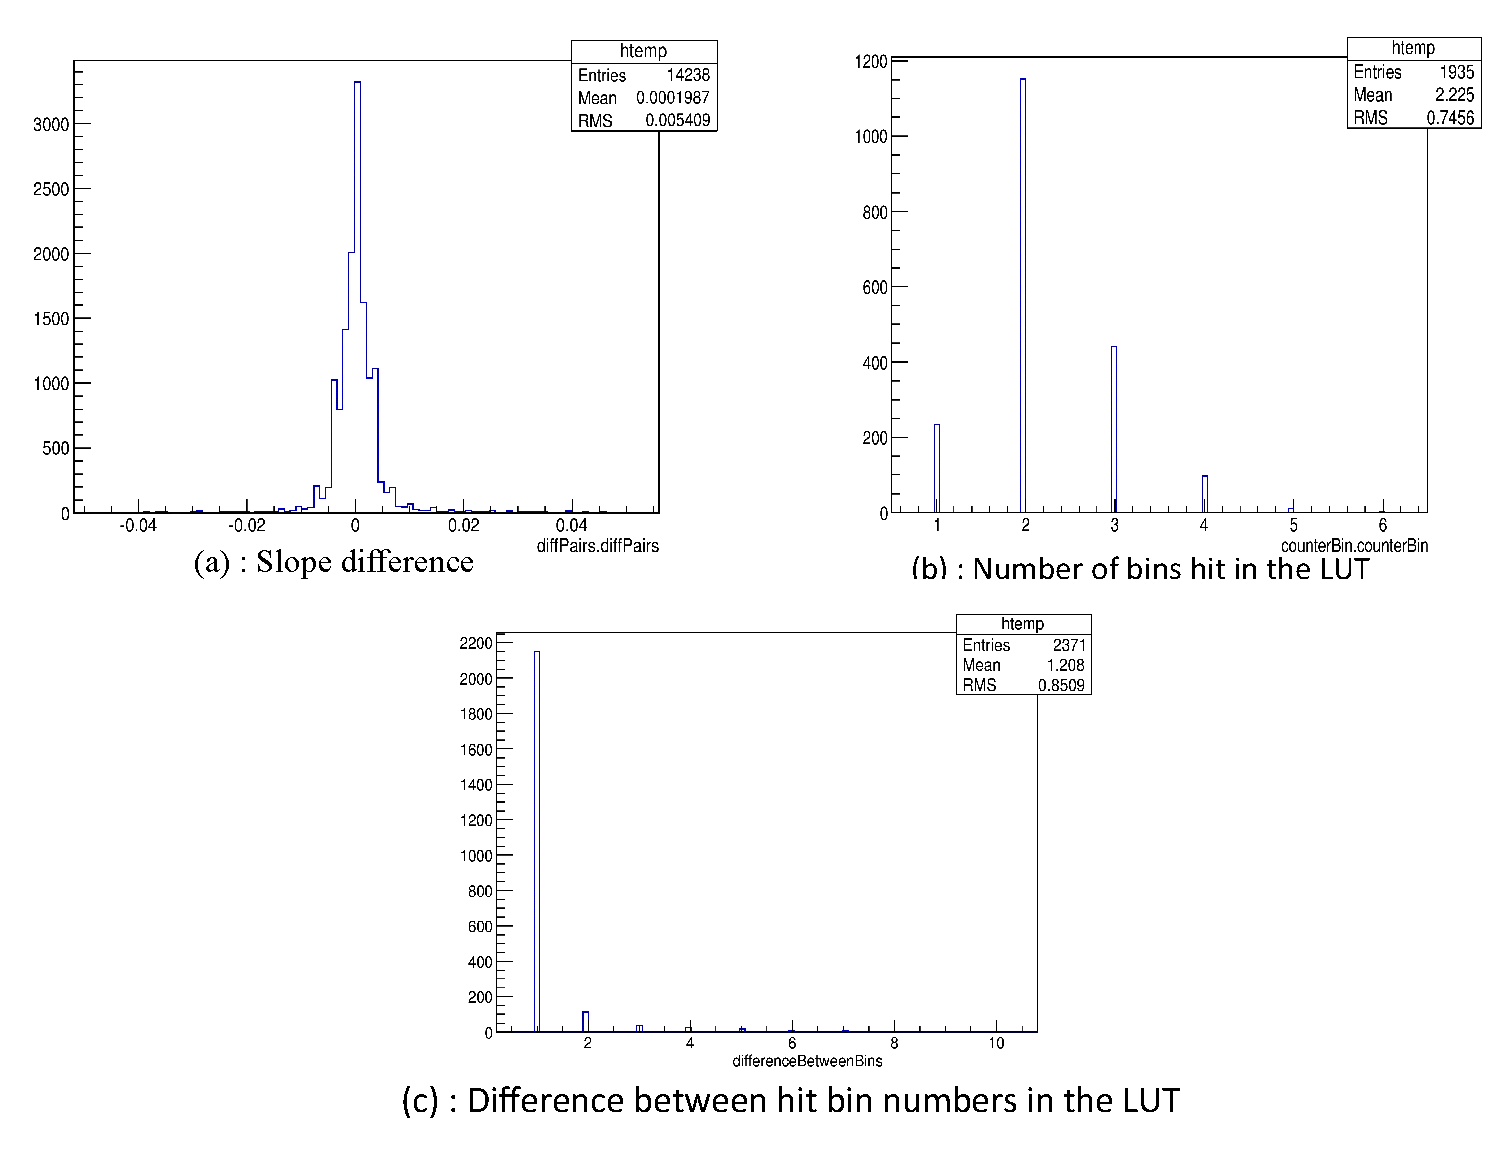
\includegraphics[width=0.99\textwidth]{algorithms-saclay/SaclayLUToptimisation.pdf}
  \caption{(a) : Difference of slope values. (b) Number of bins hit in the LUT. (c) Difference between hit bins in the LUT. }
  \label{fig:SaclayLUToptimisation}
  \end{center}
  \end{figure}
%%%%%%%%%%%%%%%%%%%%%%%%

%%%%%%%%%%%%%%
 \textbf{Intrinsic Efficiency} : The efficiency of the algorithm is defined as the ratio between the number of tracks which passed the algorithm requirement
and the total number of simulated tracks. The efficiency is calculated for the ideal case of events with eight hits (with one hit per layer).
 Figure\,\ref{fig:SaclayEfficiencyVsEtaPt}  shows the intrinsic efficiency as a function of $\eta$ and $p_{T}$
The holes observed in the efficiency distribution versus $\eta$ are explained by the gaps between the different panel regions located at $\eta \simeq 1.43, \eta \simeq 1.68$ and $\eta \simeq 2.05$. Indeed some track candidates overlap two panel regions and so cannot be taken into account by the LUT (which is defined per panel region). The global efficiency of the algorithm is 99.6\% for projective panel regions and 99.2\% otherwise. This inefficiency  cannot be fully recovered since the electronic implementation is not fully projective.
%%%%%%%%%%%%%%
  \begin{figure}[htb!]
  \centering
  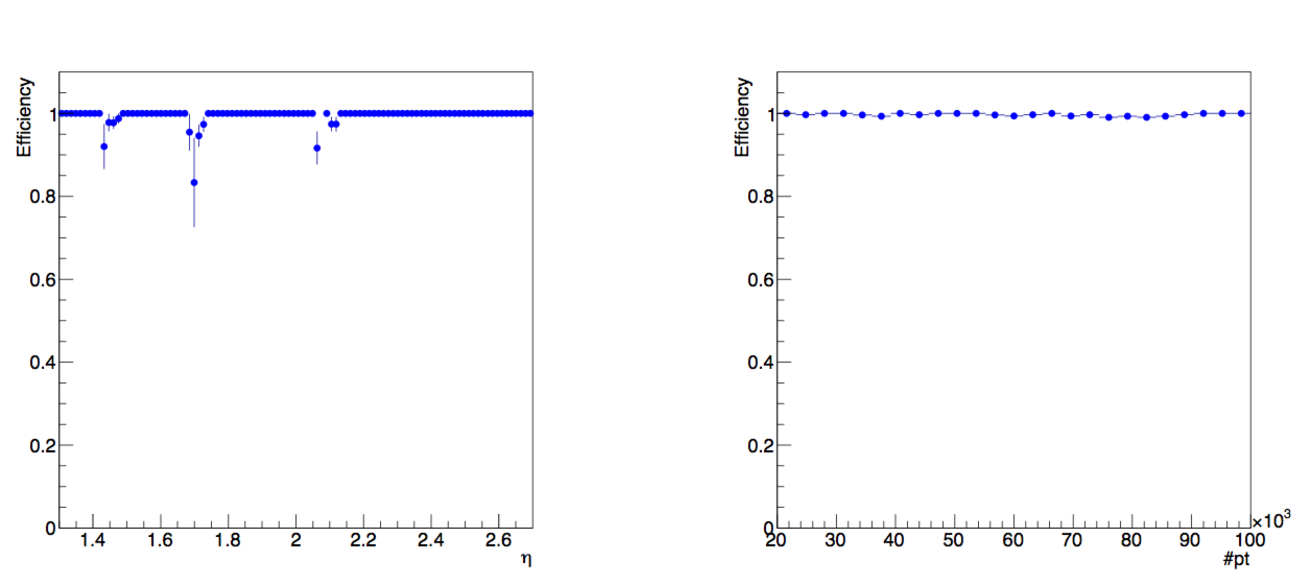
\includegraphics[width=0.95\textwidth]{algorithms-saclay/SaclayEfficiencyVsEtaPt.pdf}
  \caption{Distribution of efficiency versus $\eta$ (left) and $p_{T}$ (right) in the ideal case of eight hits (one hit per layer).}
  \label{fig:SaclayEfficiencyVsEtaPt}
  \end{figure}
%%%%%%%%%%%%%%%%%%%%%%%%

\textbf{Efficiency for six hits} : the efficiencies for  different pair requirements are shown in Figure\,\ref{fig:SaclayEfficiencyForDifferentPairRequirement}: the pairs $U$ and $V$ with four, three or two pairs $X$, and the pair $U$ or $V$ with four, three, two or one pair $X$. It is mandatory to have at least one pair $X$ to have the $\eta$ coordinate with enough precision and one of the two pairs $U$ and $V$ to determine the $\phi$ coordinate. These efficiencies are calculated in the case of only six hits (it may happens that hits are missing because the track passes through a gap between two panel regions).
For comparison, the efficiency of the Harvard algorithm with a requirement of only two layers $X$ and the layers $U$ and $V$ is of 99\%. The Saclay algorithm loses more information when hits are missing (because when one hit is missing in one layer, the pair cannot be built, so the informations of two hits is lost (and of four hits if the hit is missing on a $X$ layer), which explains this efficiency difference. However, the method of pairs should be more robust and precise for background filtering and rejection.
%%%%%%%%%%%%%%
  \begin{figure}[htb!]
  \centering
  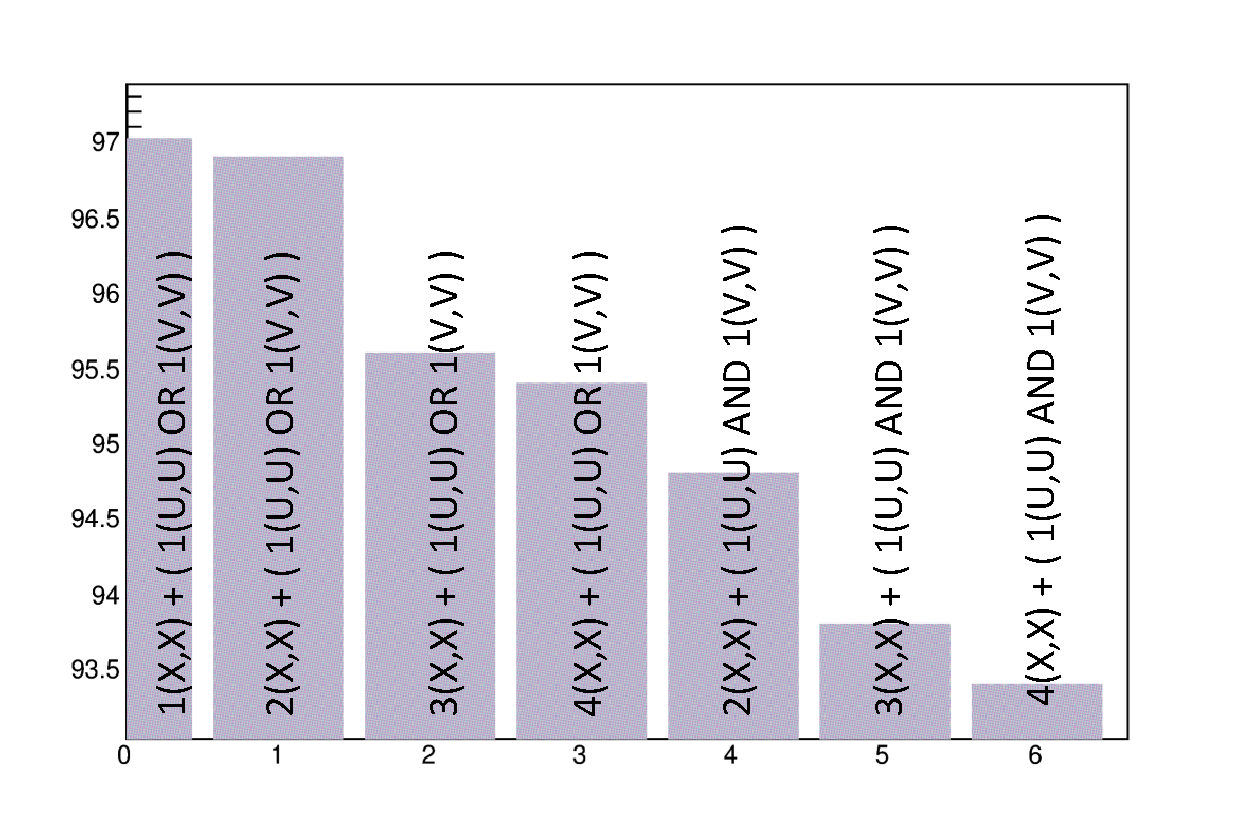
\includegraphics[width=0.55\textwidth]{algorithms-saclay/SaclayEfficiencyForDifferentPairRequirement.pdf}
  \caption{Efficiencies for different pair requirements in the case of six hits.}
  \label{fig:SaclayEfficiencyForDifferentPairRequirement}
  \end{figure}

 %%%%%%%%%%%%%
 \textbf{Resolution} : the resolution at the muon spectrometer entrance is calculated as the difference between the angle $\theta_{rec}$ as reconstructed by the algorithm and $\theta_{truth}$ as simulated at the muon spectrometer entrance. The RMS of this distribution shown in Figure\,\ref{fig:SaclayResolution} gives a resolution of 1.7\,mrad.
 %%%%%%%%%%%%%
%%%%%%%%%%%%%%
  \begin{figure}[htb!]
  \centering
  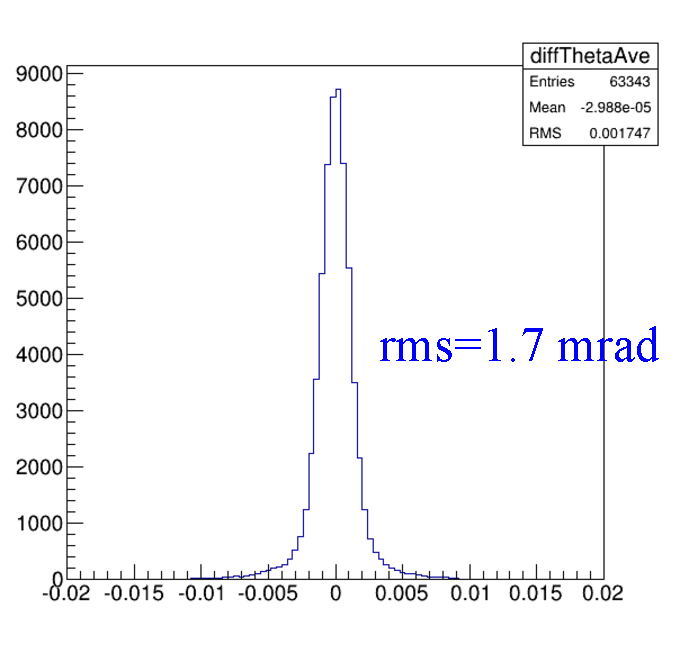
\includegraphics[width=0.45\textwidth]{algorithms-saclay/SaclayResolution.pdf}
  \caption{ $\theta$ resolution at the muon spectrometer entrance.}
  \label{fig:SaclayResolution}
  \end{figure}

 %%%%%%%%%%%%%
\textbf{Calculation of the $x$-coordinate} : What still has to be done is the calculation of the $x$-coordinate using the stereo strips and the firmware implementation. The $x$-coordinate will be used to determine the $\phi$ angle of the particle in order to build the Region of Interest characterized by
 $(\Delta\eta,\Delta\phi)$. This calculation has not been performed in this study because the stereo strips were not implemented in the simulated
samples. However, the formula that should have been used for this calculation is:
 $$\Delta X= \frac{Y_{U}-Y_{X}-\Delta Y_{\theta}}{\tan(\phi_{0})}$$
 where $Y_{U}$ is the average between the two $y$-coordinates of the hit strips of the two layers $U$, $Y_{X}$ is the average between  the two layers of one pair $X$, $\phi_{0}$ is the stereo angle ($\phi_{0}=1.5$ $^{\circ}$). The term  $\Delta Y_{\theta}=~(Z_{U}-Z_{X})\times \tan(\theta)$ (with $Z_{U}$ the average between the two $z$-coordinates of the hit strips of the two layers $U$,  $Z_{X}$ of the two layers $X$, and $\tan(\theta)$ the average of the slopes of the six pairs). This calculation, done for the four $X$ pairs once with the $U$ pair and once with the $V$ pair allows to determine the $x$-coordinate of the hits on each layer.

%%%%%%%%%%%%%%%%%%%%%%
 \subsubsubsection{Summary}
%%%%%%%%%%%%%%%%%%%%%%
The proposed algorithm for the MicroMegas New Small Wheel trigger processor, based on the Look Up Table optimization and strengthen with electronic tests, has an intrinsic efficiency of more than 99\% and can detect a particles with a precision better than 2\,mrad on the polar angle, which fulfill the requirements for the trigger. The construction of the Region of Interest of a track is still to be implemented to check if the total response time is less than 100\,ns.

The algorithm has still to be tested in presence of background which both increases the efficiency and the apparition of fakes, i.e.\ detection of muons that are in reality other products of the collision. The system of pairs should filter the background because the detection of one hit is confirmed by the hit four layers farther, and the fake particles have trajectories that are not geometrically compatible with the LUT content. However, the ionization problem and the intrinsic resolution of the detector are some limitations of the background rejection.

Recently, we have started activities on the production of cavern background simulation. This simulation can be performed using two different
approaches: one is fully based on GEANT\,4, the second is using FLUGG. Both were used in the past for simulation of physics events.
The second approach is currently under validation and the samples are expected to be produced in the next two months.
